\chapter{Formulating Scientific Hypotheses as Constraints -- A Case Study}
\label{sec:ms}

\section{Overview}
\label{sec:ms:overview}

\paragraph{Scope}

In Chapter~\ref{sec:syn}, we formally introduced constrained feature selection and evaluated the impact of randomly generated constraints in a domain-independent manner.
We observed several general trends but also noted that the results depend on the constraint types.
In this chapter, we conduct a domain-specific case study in materials science.
The solver-based optimization approach for constrained feature selection remains the same as in Chapter~\ref{sec:syn}.
However, the goal and several other components of the current study's experimental design differ significantly from the previous study.
In particular, we involve users, and the constraints represent hypotheses and user preferences (cf.~Section~\ref{sec:introduction:research-gaps:integrating-domain-knowledge}).

\paragraph{Contributions}

Our contribution in this chapter is a case study to evaluate the impact of constraints for a concrete scenario.
We use a dataset from materials science with 135 features.
The dataset represents the microstructural evolution in a material specimen subjected to tensile loading.
The physical processes behind the data are complex and currently not fully understood.
Thus, we involve domain experts as users to formulate constraints.
We evaluate domain-specific hypotheses about the data by analyzing how the corresponding constraints affect feature selection, particularly feature-set quality and the composition of feature sets.
As in the study with generated constraints (cf.~Chapter~\ref{sec:syn}), we use univariate filter feature selection as the objective, formulate constraints with propositional logic and linear arithmetic, and find optimal feature sets with an SMT solver.
Section~\ref{sec:ms:evaluation:summary} summarizes key results.

\paragraph{Materials}

We publish all our code and experimental data online (cf.~Section~\ref{sec:introduction:materials}).

\paragraph{Prior works}

The content of this chapter bases on the following prior work:
%
\begin{itemize}
	\item \fullcite{bach2022empirical}
\end{itemize}

\paragraph{Chapter outline}

The remainder of this chapter is structured as follows:
Section~\ref{sec:ms:experimental-design} outlines our experimental design, and Section~\ref{sec:ms:evaluation} presents the experimental results.

\section{Experimental Design}
\label{sec:ms:experimental-design}

In this section, we introduce our experimental design for the case study in materials science.
First, we give a brief overview (cf.~Section~\ref{sec:ms:experimental-design:overview}).
Next, we present our scenario and dataset (cf.~Section~\ref{sec:ms:experimental-design:scenario}), objective function (cf.~Section~\ref{sec:ms:experimental-design:objective}), constraint types (cf.~Section~\ref{sec:ms:experimental-design:constraints}), evaluation metrics (cf.~Section~\ref{sec:ms:experimental-design:metrics}), and prediction models (cf.~Section~\ref{sec:ms:experimental-design:prediction}).
Finally, we briefly outline our implementation (cf.~Section~\ref{sec:ms:experimental-design:implementation}).

\subsection{Overview}
\label{sec:ms:experimental-design:overview}

In this case study, we evaluate constraints on one dataset from materials science.
In particular, we analyze twelve constraint types representing hypotheses from the domain and also add three domain-independent constraint types representing user preferences.
As in the study with generated constraints, we employ the objective of univariate filter feature selection.
We evaluate feature-set quality and the composition of the feature sets.

\subsection{Scenario and Dataset}
\label{sec:ms:experimental-design:scenario}

We collaborate with materials scientists who provide us with a dataset and act as domain experts for formulating constraints and interpreting results.
The general scenario of our study involves crystalline materials, such as most metals, on the micro-scale.
These materials incorporate defect structures, i.e., dislocations, within the regular crystal structure.
The line-like dislocations evolve over time and build complex 3D networks, which are mainly responsible for the permanent deformation of the material under load.
Understanding the network evolution is vital in characterizing the deformation behavior. 

The particular dataset in our study represents an aluminum specimen under tensile load~\cite{sudmanns2020data}.
Our domain experts created the dataset with numerical simulations using the method of discrete dislocation dynamics~\cite{weygand2001discrete}.
From a materials-science perspective, the research aims to study the evolution of properties characterizing the dislocation network.
An example of such a property is the slip system, i.e., the slip plane and slip direction in which a dislocation can move.
In face-centered cubic crystals, like our specimen, there are twelve slip systems.
Another example is the so-called Schmid factor.
It characterizes the slip plane and the slip direction that resolves the highest mechanical stress. 

\begin{table}[t]
	\centering
	\caption{
		Physical quantities and features in the materials-science dataset.
	}
	\begin{tabular}{llrrr}
		\toprule
		Base quantity & Symbol & Slip systems & Aggregates & Features \\
		\midrule
		edge\_resolved\_shear & $\sigma_\text{rss}^\text{edge}$ &            12 &           5 &        17 \\
		eps\_equiv & $\varepsilon_\text{eq}^\text{pl}$ &              0 &           0 &         1 \\
		eps\_xx & $\varepsilon_\text{xx}^\text{pl}$ &              0 &           0 &         1 \\
		eps\_xy & $\varepsilon_\text{xy}^\text{pl}$ &              0 &           0 &         1 \\
		eps\_xz & $\varepsilon_\text{xz}^\text{pl}$ &              0 &           0 &         1 \\
		eps\_yy & $\varepsilon_\text{yy}^\text{pl}$ &              0 &           0 &         1 \\
		eps\_yz & $\varepsilon_\text{yz}^\text{pl}$ &              0 &           0 &         1 \\
		eps\_zz & $\varepsilon_\text{zz}^\text{pl}$ &              0 &           0 &         1 \\
		free\_path\_per\_voxel & $\overline{l}_\text{norm}$ &              0 &           0 &         1 \\
		gamma & $\gamma$ &             12 &           5 &        17 \\
		gamma\_abs & $\gamma_\text{abs}$ &             12 &           5 &        17 \\
		kappa1 & $\kappa_\text{screw}$ &             12 &           5 &        17 \\
		kappa2 & $\kappa_\text{edge}$ &             12 &           5 &        17 \\
		mean\_free\_path & $\overline{l}$ &              0 &           0 &         1 \\
		n\_loops & $n_\text{loops}$ &              0 &           0 &         1 \\
		pos\_x & $x$ &              0 &           0 &         1 \\
		pos\_y & $y$ &              0 &           0 &         1 \\
		pos\_z & $z$ &              0 &           0 &         1 \\
		q & $q$ &             12 &           5 &        17 \\
		rho & $\rho$ &             12 &           5 &        17 \\
		step & -- &              0 &           0 &         1 \\
		time & $t$ &              0 &           0 &         1 \\
		vonMises & $\sigma_\text{vM}$ &              0 &           0 &         1 \\
		\bottomrule
	\end{tabular}
	\label{tab:ms:features}
\end{table}

Dislocation lines can react with each other in several ways.
Our prediction target is the density of dislocation line segments attached to so-called glissile reactions.
Table~\ref{tab:ms:features} gives an overview of the features in the dataset, which are other physical quantities of the system, like dislocation density, shear stress, etc.
Overall, the dataset consists of 14903 data objects and 135 features.
Each data object represents the state of the material specimen at a particular location and time step.
For predictions, we exclude the features for location, time, and simulation-step size, which leaves 130 features.
As Table~\ref{tab:ms:features} displays, some physical quantities correspond to one feature, while others yield 17 features.
In particular, some quantities in our dataset are measured separately for each of the twelve slip systems.
In this case, we also compute five aggregates, i.e., the minimum, maximum, median, sum, and standard deviation over the twelve slip systems.

\subsection{Objective Function and Optimization}
\label{sec:ms:experimental-design:objective}

As in the study with generated constraints (cf.~Section~\ref{sec:syn:experimental-design:objective}), we use the SMT solver \emph{Z3} \cite{bjorner2015nuz, deMoura2008z3} to optimize the univariate objective from Equation~\ref{eq:fs:univariate-filter}.
To instantiate the dependency measure~$q(\cdot)$, we take the absolute values of the Pearson correlation of each feature with the target variable, rather than the mutual information used in Chapter~\ref{sec:syn}.
In particular, preliminary experiments showed strong linear relationships in the data.
Also, the constraint types~\ref{enum:ms:constraint-type:inter-correlation} and~\ref{enum:ms:constraint-type:quality-filter}, which we introduce in the next section, assume that the dependency measure $q(\cdot)$ is bounded to $[0, 1]$, which mutual information violates.

\subsection{Constraints}
\label{sec:ms:experimental-design:constraints}

\paragraph{Overview}

This case study aims to evaluate the impact of constraints on feature selection in a concrete use case.
We did not identify firm domain knowledge suited for constraints.
However, we can still formulate constraints about hypothesized relationships between features.
We then evaluate how the resulting feature sets and feature-set quality change compared to an unconstrained selection.
Several outcomes are possible.
For example, the selected features may change, but the feature-set quality remains similar, indicating an alternative explanation.
Instead, feature-set quality may drop, indicating that the hypothesis behind the constraints is wrong.
By formulating different sets of constraints and evaluating them independently, one can also compare different hypotheses.

Besides domain-specific constraints representing the hypotheses, we also employ domain-independent constraints expressing preferences on the resulting feature sets.
As in our study with generated constraints (cf.~Chapter~\ref{sec:syn}), each constraint type may be formulated in multiple, logically equivalent ways.
In the following, we present one formulation each.

\paragraph{Domain-independent constraint types}

In preliminary experiments, we observed three phenomena that made it difficult for domain experts to interpret feature sets.
These phenomena were neither specific to our case study nor the domain in general.
We use three constraint types to alleviate these phenomena:
%
\begin{enumerate}[label=(I\arabic*), wide]
	\item\label{enum:ms:constraint-type:global-cardinality} \emph{Global-cardinality}:
	Larger feature sets may be harder to interpret for domain experts.
	Thus, we apply a global cardinality constraint, which is the same as~\ref{enum:syn:constraint-type:global-at-most} from the previous chapter.
	Here, we apply thresholds of $k \in \{5, 10\}$ features, so we can also compare how the feature-set quality changes from the smaller to the larger cardinality.
	%
	\begin{equation}
		\text{Global-cardinality}(\{s_1, \dots, s_n\}, k) =\\
		\sum_{j=1}^{n} s_j \leq k \text{, with } k \in \{5,10\}
		\label{eq:ms:constraint:global-cardinalty}
	\end{equation}
	%
	\item\label{enum:ms:constraint-type:inter-correlation} \emph{Inter-correlation}:
	Datasets may contain features strongly correlated with each other.
	Having such highly correlated features in the result may be undesirable, e.g., if they describe the same physical phenomenon, only measured or encoded differently.
	However, the objective function in Equation~\ref{eq:fs:univariate-filter} considers features independently, thus ignoring inter-feature correlation.
	Thus, we employ a correlation threshold:
	If a pair of features has an absolute Pearson correlation of at least $\tau = 0.8$, we select at most one of these features.
	The correlation values~$q(X_{\cdot{}j_1},X_{\cdot{}j_2})$ for each pair of features $j_1$,~$j_2$ can be precomputed and are therefore constants in the following formula, as is the user parameter~$\tau$.
	%
	\begin{multline}
		\text{Inter-correlation}(\{s_1, \dots, s_n\}, \tau) = \bigwedge_{\substack{(j_1, j_2) \in \{1, \dots, n\}^2 \\ j_1 \neq j_2}} \left( \left( q(X_{\cdot{}j_1},X_{\cdot{}j_2}) \geq \tau \right) \rightarrow \lnot (s_{j_1} \land s_{j_2}) \right)\\
		\text{with } \tau = 0.8
		\label{eq:ms:constraint:inter-correlation}
	\end{multline}
	%
	\item\label{enum:ms:constraint-type:quality-filter} \emph{Quality-filter}:
	Datasets may contain features with a quality close to zero.
	These features provide little value when being selected but may increase optimization time.
	Thus, it makes sense to remove such features manually before optimization or to add a respective constraint.
	We set a quality threshold of 0.2 and exclude features with a lower quality.
	The feature qualities~$q(X_{\cdot{}j},y)$ and the threshold $\tau$ are constants.
	%
	\begin{equation}
		\text{Quality-filter}(\{s_1, \dots, s_n\}, \tau) =\\
		\bigwedge_{j=1}^{n} \left( \left( q(X_{\cdot{}j},y) < \tau \right) \rightarrow \lnot s_j \right) \text{, with } \tau = 0.2
		\label{eq:ms:constraint:quality-filter}
	\end{equation}
	%
\end{enumerate}

\paragraph{Domain-specific constraint types}

The following constraint types express hypotheses:
%
\begin{enumerate}[label=(D\arabic*), wide]
	\item\label{enum:ms:constraint-type:schmid-group} \emph{Schmid-group}:
	For the crystal orientation of the considered specimen, the twelve slip systems can be divided into two non-overlapping groups based on the Schmid factor.
	Let $\mathbb{G}$ be this partitioning, i.e., a set of sets with $|\mathbb{G}| = 2$.
	We hypothesize that having features from at most one of these groups should suffice.
	Within the chosen group, an arbitrary number of features can be selected.
	To formalize this notion, let $P$ be the set of physical quantities measured for the twelve slip systems (cf.~Table~\ref{tab:ms:features}).
	Further, let the subscript $(p,g)$ identify a feature derived for a physical quantity $p$ and a slip system $g$.
	%
	\begin{equation}
		\text{Schmid-group}(\{s_1, \dots, s_n\}) = \sum_{G \in \mathbb{G}} \left( \bigvee_{p \in P,~g \in G} s_{(p,g)} \right) \leq 1
		\label{eq:ms:constraint:schmid-group}
	\end{equation}
	%
	\item\label{enum:ms:constraint-type:quantity-schmid-group} \emph{Quantity-Schmid-group}:
	The constraint type~\ref{enum:ms:constraint-type:schmid-group} goes over all physical quantities.
	Alternatively, one can choose between the two slip-system groups for each quantity independently.
	With such a constraint, we hypothesize that one slip-system group may be relevant for some quantities and the other group for other quantities.
	This constraint type makes feature selection more flexible, i.e., the hypothesis is less strict.
	%
	\begin{equation}
		\text{Quantity-Schmid-group}(\{s_1, \dots, s_n\}) = \bigwedge_{p \in P} \left( \sum_{G \in \mathbb{G}} \left( \bigvee_{g \in G} s_{(p,g)} \right) \leq 1 \right)
		\label{eq:ms:constraint:quantity-schmid-group}
	\end{equation}
	%
	\item\label{enum:ms:constraint-type:schmid-group-representative} \emph{Schmid-group-representative}:
	Using the grouping of~\ref{enum:ms:constraint-type:schmid-group}, one can also select at most one feature from each group instead of selecting features from at most one group.
	This constraint type corresponds to the situation where both groups are important, but it is sufficient to pick a representative feature in each group.
	%
	\begin{equation}
		\text{Schmid-group-representative}(\{s_1, \dots, s_n\}) = \bigwedge_{G \in \mathbb{G}} \left( \sum_{p \in P,~g \in G} s_{(p,g)} \leq 1 \right)
		\label{eq:ms:constraint:schmid-group-representative}
	\end{equation}
	%
	\item\label{enum:ms:constraint-type:quantity-schmid-group-representative} \emph{Quantity-Schmid-group-representative}:
	We merge the ideas of \ref{enum:ms:constraint-type:quantity-schmid-group} and \ref{enum:ms:constraint-type:schmid-group-representative}:
	For each quantity independently, select at most one feature per slip-system group.
	%
	\begin{equation}
		\text{Quantity-Schmid-group-representative}(\{s_1, \dots, s_n\}) = \bigwedge_{p \in P,~G \in \mathbb{G}} \left( \sum_{g \in G} s_{(p,g)} \leq 1 \right)
		\label{eq:ms:constraint:quantity-schmid-group-representative}
	\end{equation}
	%
	\item\label{enum:ms:constraint-type:plastic-strain-tensor} \emph{Plastic-strain-tensor}:
	Six features in our dataset describe the plastic strain tensor, corresponding to six different directions in space.
	These are the quantities starting with \emph{eps\_} in Table~\ref{tab:ms:features}, excluding \emph{eps\_quiv}.
	We hypothesize that selecting three of the six directions should be sufficient.
	To formalize this notion, let $T$ be a set of indices, identifying features that describe the plastic strain tensor.
	%
	\begin{equation}
		\text{Plastic-strain-tensor}(\{s_1, \dots, s_n\}) = \sum_{t \in T} s_t \leq 3
		\label{eq:ms:constraint:plastic-strain-tensor}
	\end{equation}
	%
	\item\label{enum:ms:constraint-type:dislocation-density} \emph{Dislocation-density}:
	In our dataset, several features describe dislocation density aggregated over all slip systems:
	the five standard aggregates of \emph{rho} as well as the quantities \emph{free\_path\_per\_voxel} and \emph{mean\_free\_path} (cf.~Table~\ref{tab:ms:features}).
	We hypothesize that selecting at most one such feature is sufficient.
	To formalize this notion, let $D$ be a set of indices, identifying features that describe dislocation density aggregated over all slip systems.
	%
	\begin{equation}
		\text{Dislocation-density}(\{s_1, \dots, s_n\}) = \sum_{d \in D} s_d \leq 1
		\label{eq:ms:dislocation-density}
	\end{equation}
	%
	\item\label{enum:ms:constraint-type:plastic-strain-rate} \emph{Plastic-strain-rate}:
	For the plastic strain rate, our dataset contains features originating from two different computation methods.
	These quantities are named \emph{gamma} and \emph{gamma\_abs} in Table~\ref{tab:ms:features}.
	We hypothesize that selecting features from at most one method should suffice.
	To formalize this notion, let $R_1$ and $R_2$ be sets of indices, identifying features originating from the two computation methods.
	%
	\begin{equation}
		\text{Plastic-strain-rate}(\{s_1, \dots, s_n\}) = \left( \bigvee_{r \in R_1} s_{r} \right) + \left( \bigvee_{r \in R_2} s_{r} \right) \leq 1
		\label{eq:ms:plastic-strain-rate}
	\end{equation}
	%
	\item\label{enum:ms:constraint-type:aggregate} \emph{Aggregate}:
	We have aggregated several physical quantities over the twelve slip systems (cf.~Table~\ref{tab:ms:features}).
	However, the five aggregate functions may be redundant to each other.
	Thus, we hypothesize that at most one kind of aggregate should suffice.
	To formalize this notion, let $P$ be the set of physical quantities measured for the twelve slip systems and let $A$ be the set of aggregate functions.
	Further, let subscript $(p,a)$ identify a feature derived for a physical quantity $p$ and an aggregate function $a$.
	%
	\begin{equation}
		\text{Aggregate}(\{s_1, \dots, s_n\}) = \sum_{a \in A} \left( \bigvee_{p \in P} s_{(p,a)} \right) \leq 1
		\label{eq:ms:constraint:aggregate}
	\end{equation}
	%
	\item\label{enum:ms:constraint-type:quantity-aggregate} \emph{Quantity-aggregate}:
	Constraint type~\ref{enum:ms:constraint-type:aggregate} can be refined to choose the aggregate function for each physical quantity independently.
	This new constraint type allows choosing different aggregate functions for different quantities.
	%
	\begin{equation}
		\text{Quantity-aggregate}(\{s_1, \dots, s_n\}) = \bigwedge_{p \in P} \left( \sum_{a \in A} s_{(p,a)} \leq 1 \right)
		\label{eq:ms:constraint:quantity-aggregate}
	\end{equation}
	%
	\item\label{enum:ms:constraint-type:aggregate-or-original} \emph{Aggregate-or-original}:
	Aggregates describe the same physical quantities as the features they aggregate.
	Thus, we hypothesize that selecting original features or aggregates for each quantity should suffice.
	To formalize this notion, let subscript $(p,l)$ identify a feature derived for a physical quantity $p$ and a slip system $l \in \{1, \dots, 12\}$.
	%
	\begin{equation}
		\text{Aggregate-or-original}(\{s_1, \dots, s_n\}) = \bigwedge_{p \in P} \left( \left( \bigvee_{a \in A} s_{(p,a)} \right) + \left( \bigvee_{l \in \{1, \dots, 12\}} s_{(p,l)} \right) \leq 1 \right)
		\label{eq:ms:aggregate-or-original}
	\end{equation}
	%
	\item\label{enum:ms:constraint-type:mixed} \emph{Mixed}:
	Various combinations of the previous constraint types above are possible, though some constraint types are redundant or compete with each other.
	For comparison, we consider the union of \ref{enum:ms:constraint-type:quantity-schmid-group-representative}, \ref{enum:ms:constraint-type:plastic-strain-tensor}, \ref{enum:ms:constraint-type:dislocation-density}, \ref{enum:ms:constraint-type:plastic-strain-rate}, \ref{enum:ms:constraint-type:quantity-aggregate}, and \ref{enum:ms:constraint-type:aggregate-or-original}.
	%
	\begin{equation}
		\begin{aligned}
			\text{Mixed}(\{s_1, \dots, s_n\}) &=~\text{Quantity-Schmid-group-representative}(\{s_1, \dots, s_n\}) \land \\
			& \text{Plastic-strain-tensor}(\{s_1, \dots, s_n\}) \land \\
			& \text{Dislocation-density}(\{s_1, \dots, s_n\}) \land \\
			& \text{Plastic-strain-rate}(\{s_1, \dots, s_n\}) \land \\
			& \text{Quantity-aggregate}(\{s_1, \dots, s_n\}) \land \\
			& \text{Aggregate-or-original}(\{s_1, \dots, s_n\})
		\end{aligned}
		\label{eq:ms:constraint:mixed}
	\end{equation}
	%
	\item\label{enum:ms:constraint-type:unconstrained} \emph{Unconstrained}:
	As a reference point, we evaluate the setting without domain-specific constraints.
	This definition is the same as~\ref{enum:syn:constraint-type:unconstrained} in the previous chapter.
	%
	\begin{equation}
		\text{Unconstrained}(\{s_1, \dots, s_n\}) = 1
		\label{eq:ms:constraint:unconstrained}
	\end{equation}
	%
\end{enumerate}

\paragraph{Combining domain-independent and domain-specific constraint types}

We create two sets of constraints from the domain-independent constraint types \ref{enum:ms:constraint-type:global-cardinality}, \ref{enum:ms:constraint-type:inter-correlation}, and \ref{enum:ms:constraint-type:quality-filter}.
Both sets involve all three types, but one uses the feature-set cardinality $k=5$, and the other $k=10$.
We combine each of these two constraint sets with each of the twelve domain-specific constraint types.
Thus, we get 24 constraint sets overall.
In the following evaluation, we mainly mention the names of the domain-specific constraint types, but the domain-independent constraint types are always active as well.

\subsection{Evaluation Metrics}
\label{sec:ms:experimental-design:metrics}

To evaluate our hypotheses expressed as constraints, we focus on selected features and feature-set quality, i.e., objective value and prediction performance.
In particular, we analyze how these outcomes differ between hypotheses.
Technically, we could use the complete set of evaluation metrics from the study with generated constraints (cf.~Section~\ref{sec:syn:experimental-design:metrics}).
However, we only have 24 experimental runs here, so statements on the relationship between evaluation metrics would be less generalizable.

\subsection{Prediction}
\label{sec:ms:experimental-design:prediction}

We use the same prediction models as in the study with generated constraints (cf.~Section~\ref{sec:syn:experimental-design:prediction}).
As our current dataset has a temporal dimension, we apply a time-based 80:20 holdout split instead of cross-validation,
i.e., all data objects in the training data are from earlier time steps than in the test data.
However, our predictions do not go into the future.
Instead, we predict the target variable from feature values at the same time step.

\subsection{Implementation and Execution}
\label{sec:ms:experimental-design:implementation}

As in the previous study (cf.~Section~\ref{sec:syn:experimental-design:implementation}), we implemented our experimental pipeline in Python~3.7, using \emph{scikit-learn}~\cite{pedregosa2011scikit-learn} and \emph{xgboost}~\cite{chen2016xgboost} for machine learning and the SMT solver \emph{Z3}~\cite{bjorner2015nuz, deMoura2008z3} for optimization.
All code is available online (cf.~Section~\ref{sec:introduction:materials}).
We organized the constrained-feature-selection functionality as a Python package.

Our experimental pipeline parallelizes over constraint types, while each of these experimental tasks runs single-threaded.
We ran the pipeline on a server with 128~GB RAM and an \emph{AMD EPYC 7551} CPU, having 32~physical cores and a base clock of 2.0~GHz.
With this hardware, the parallelized pipeline run took less than one hour.

\section{Evaluation}
\label{sec:ms:evaluation}

In this section, we evaluate our case study in materials science.
In particular, we analyze feature-set quality (cf.~Section~\ref{sec:ms:evaluation:quality}) and selected features (cf.~Section~\ref{sec:ms:evaluation:features}).
Finally, we summarize key findings (cf.~Section~\ref{sec:ms:evaluation:summary}).

\subsection{Feature-Set Quality}
\label{sec:ms:evaluation:quality}

\begin{figure}[t]
	\centering
	\begin{subfigure}{0.48\textwidth}
		\centering
		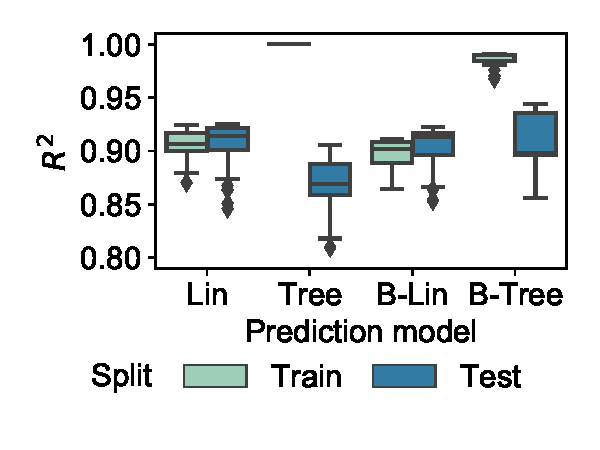
\includegraphics[width=\textwidth, trim=15 25 15 15, clip]{plots/ms-prediction-performance-split.pdf}
		\caption{All data, by split.}
		\label{fig:ms:prediction-performance-split}
	\end{subfigure}
	\hfill
	\begin{subfigure}{0.48\textwidth}
		\centering
		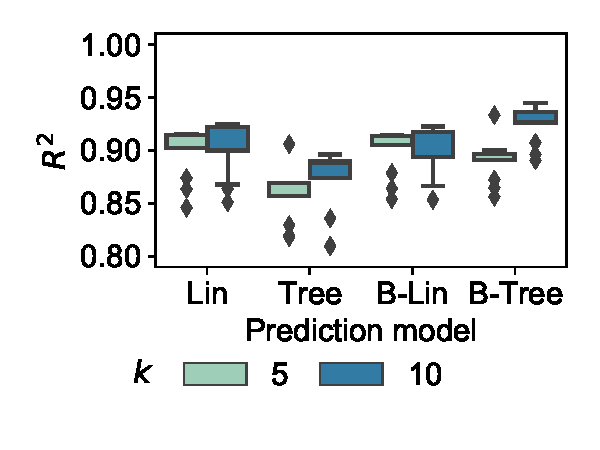
\includegraphics[width=\textwidth, trim=15 25 15 15, clip]{plots/ms-prediction-performance-cardinality.pdf}
		\caption{Only test data, by cardinality~$k$.}
		\label{fig:ms:prediction-performance-cardinality}
	\end{subfigure}
	\caption{Distribution of prediction performance over constraint types, by prediction model.}
	\label{fig:ms:prediction-performance}
\end{figure}

\paragraph{Prediction performance}

Figure~\ref{fig:ms:prediction-performance-split} shows the prediction performance over all 24 experimental runs.
All four prediction models perform well, even simple linear regression.
The twelve domain-specific constraint types cause some but not substantial variation in prediction performance.
Figure~\ref{fig:ms:prediction-performance-cardinality} shows that models with five features tend to perform only slightly worse than models with ten features.
I.e., one can make good predictions with a small set of features, which renders the scenario suitable for feature selection.

\paragraph{Objective value}

The objective value, i.e., summed univariate feature quality (cf.~Section~\ref{sec:ms:experimental-design:objective}), is also high and has a relatively low variance over constraint types.
In particular the objective value is in $[3.79, 4.04]$ for $k=5$ features and in $[6.45, 7.48]$ for $k=10$.
The theoretical upper bound on each feature's quality is~1.
In our dataset, the maximum feature quality is 0.92, and the average feature quality is 0.27.
Thus, the objective values achieved are considerably higher than the expected values, i.e.,
$0.27\cdot 5=1.35$ and $0.27 \cdot 10=2.7$.

The constraint type \emph{Mixed}~\ref{enum:ms:constraint-type:mixed} yields the lowest objective value for both cardinalities.
This type combines six other constraint types and thus restricts the search space more than the others.
Without this constraint type, the ranges of the objective value narrow down to $[3.92, 4.04]$ and $[7.03, 7.48]$.
I.e., our domain-specific constraint types have relatively little impact on the objective value.
In contrast, cardinality does have a noticeable impact, as can be expected from the linear objective.
Nevertheless, the size of the increase indicates that the sixth to tenth selected features still have relatively high quality.
This result should give way to alternative feature sets with similar quality, as we analyze later.

\paragraph{Comparing hypotheses}

As none of the analyzed constraint types significantly decrease feature-set quality, none of the underlying hypotheses seem to be invalidated.
Further, the modest variation of feature-set quality between hypotheses makes it challenging to draw conclusions regarding individual hypotheses.
A more detailed, domain-specific analysis of the hypotheses may be beneficial but is beyond the scope of this dissertation.

\subsection{Selected Features}
\label{sec:ms:evaluation:features}

\begin{figure}[t]
	\centering
	\begin{subfigure}{0.48\textwidth}
		\centering
		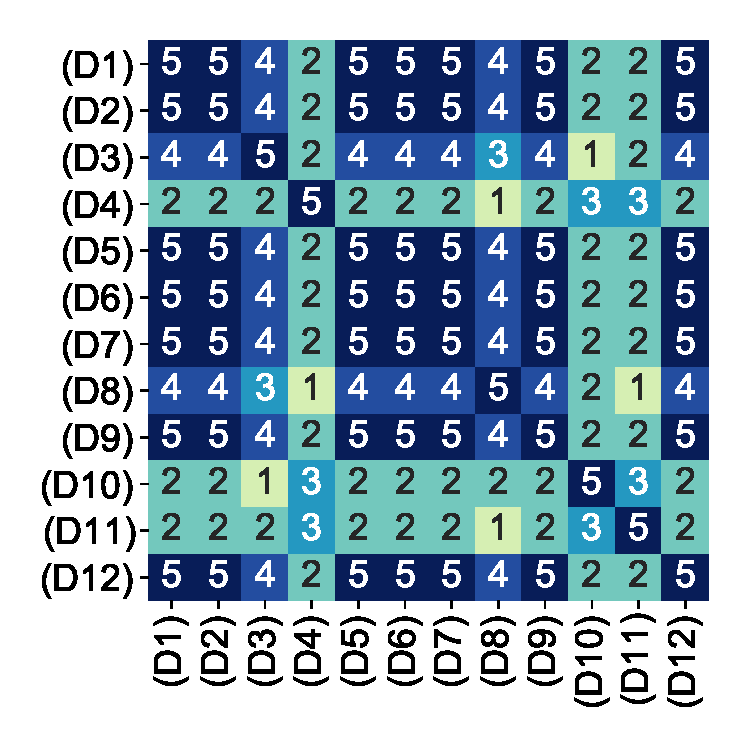
\includegraphics[width=\textwidth, trim=15 15 15 15, clip]{plots/ms-selected-similarity-card5.pdf}
		\caption{Cardinality $k=5$.}
		\label{fig:ms:selected-similarity-card5}
	\end{subfigure}
	\hfill
	\begin{subfigure}{0.48\textwidth}
		\centering
		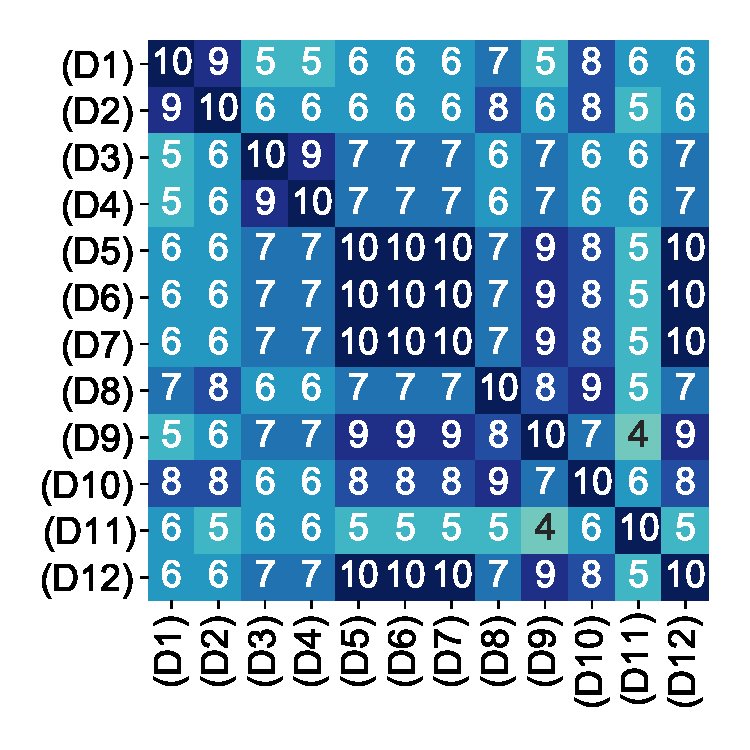
\includegraphics[width=\textwidth, trim=15 15 15 15, clip]{plots/ms-selected-similarity-card10.pdf}
		\caption{Cardinality $k=10$.}
		\label{fig:ms:selected-similarity-card10}
	\end{subfigure}
	\caption{Number of common features between resulting feature sets for different constraint types.}
	\label{fig:ms:selected-similarity}
\end{figure}

For all constraint types, the selected feature sets contain several dislocation-density-related features.
This observation is expected, as the target variable quantifies reactions of dislocations.
Figure~\ref{fig:ms:selected-similarity} shows how many selected features are the same when comparing results with different constraint types.
For $k=5$ (cf.~Figure~\ref{fig:ms:selected-similarity-card5}), several constraint types share more than half of their selected features.
In particular, six constraint types yield the same feature set as the reference case, i.e., \emph{Unconstrained}~\ref{enum:ms:constraint-type:unconstrained}.
We see two reasons for such `inactive' constraints.
First, the constraints may already be consistent with the unconstrained result even if they refer to its features.
For example, \emph{Unconstrained}~\ref{enum:ms:constraint-type:unconstrained} with $k=5$ only selects dislocation-density features from one slip-system group, so the constraint types \emph{Schmid-group}~\ref{enum:ms:constraint-type:schmid-group} and \emph{Quantity-Schmid-group}~\ref{enum:ms:constraint-type:quantity-schmid-group} are satisfied already.
Second, some constraint types may not affect any of the selected features in the reference case.
For example, \emph{Plastic-strain-rate}~\ref{enum:ms:constraint-type:plastic-strain-rate} and \emph{Plastic-strain-tensor}~\ref{enum:ms:constraint-type:plastic-strain-tensor} refer to physical quantities that have low quality in the prediction scenario. 
In future work, one might apply an iterative approach to avoid inactive constraints:
inspect the unconstrained result, formulate constraints, inspect the results, etc.

The picture becomes slightly more diverse for $k=10$ (cf.~Figure~\ref{fig:ms:selected-similarity-card10}).
Most constraint types still share at least half the selected features.
However, there are fewer cases where all features are the same since the reference case violates more constraint types now.
Still, as observed in the previous section, the feature-set quality is pretty similar between the constraint types.
For example, \emph{Mixed}~\ref{enum:ms:constraint-type:mixed} swaps 3/5 or 5/10 features compared to \emph{Unconstrained}~\ref{enum:ms:constraint-type:unconstrained}.
At the same time, the objective value only drops by 6.2\% or 13.8\%, which is a much smaller share.
This observation indicates that constraints may yield alternative feature sets that differ from the reference case but still have a similar quality.

\subsection{Summary}
\label{sec:ms:evaluation:summary}

We observed that our domain-specific constraint types had a relatively small impact on feature-set quality.
In other words, our analysis did not yield evidence against our hypotheses.
However, constraints resulted in features being replaced with alternatives of similar quality, motivating a principled approach for alternative feature selection (cf.~Chapter~\ref{sec:afs}).
Also, selecting only a few features sufficed to reach a high prediction performance.
Additionally, several constraint types were already satisfied in the solution of the unconstrained reference case.
Thus, we recommend an iterative approach of inspecting solutions and formulating new constraints instead of formulating all constraints upfront.
